% !Rnw root = Introduction.Rnw
\section{Using R}
\subsection{An Interactive Session}
\begin{HIGHLIGHT}
\par\noindent{
R is an \emph{interactive} environment, wherein the users gets immediate feedback (\emph{results}) for their instructions (\emph{expressions}). This is in contrast to programming languages like C++ or Java wherein a set of instructions (the program) has to be created and compiled before the results can be generated.In R, the interaction between the user and the system constitutes an \emph{R Session}. During an R session, the user provides \emph{expressions} to R for doing computations, displaying results, and creating objects for further use. R, first evaluates the expressions for its syntactic correctness and then performs the task, as specified by the expression. We will examine some basic expressions in the next section.     
}
\end{HIGHLIGHT}

\begin{HIGHLIGHT}
\par\noindent{
R, like Python, MATLAB etc is a \emph{dynamically typed language} which means that you won't have to define the type of the variable (which stores your data). As a result, the user can only focus on the \emph{data stored by the variable} rather than having to worry about \emph{how the data is stored in the variable}. This is in stark contrast to \emph{statically typed languages} like C++ and Java.      
}
\end{HIGHLIGHT}

\begin{DIY}{Think}
How does a R \emph{data frame} exemplify the \emph{dynamic typing} feature of R?
\end{DIY}
    
\begin{DIY}{Warning}
The dynamic typing feature of R  provides great flexibility but at what cost?
\end{DIY}



% !Rnw root = UsingR.Rnw
%==================================  
\subsection{Basic Expressions in R}
%==================================  
At the \emph{console}, the user finds the \textbf{$>$} prompt where the user responds by typing and expression. Hereon, in this section every expression/set of expressions is mentioned in the gray box and is to be issued at the $>$ prompt in the console. Moreover, following the motto of this course ``learn by doing``, the reader is strongly encouraged to try out each of these expressions and \emph{read the corresponding help manual for each expression}. As is evident from the examples shown in this section, expressions are predominantly \textbf{\emph{function calls with a set of arguments}}.

\begin{HIGHLIGHT}
\par\noindent{
Objects are the center of computations in R, along with the function calls that create and use those objects.
}
\end{HIGHLIGHT}

\begin{DIY}{Think}
What are objects in R? Why are functions and objects dual to each other? 
\end{DIY}

%==================================  
\subsubsection{Want Help?: Use the ``\textbf{?}'' operator}
%==================================  
\noindent The \textbf{?} operator displays help for the topic that follows it.
\begin{knitrout}
\definecolor{shadecolor}{rgb}{0.969, 0.969, 0.969}\color{fgcolor}\begin{kframe}
\begin{alltt}
\hlopt{?}\hlstd{data.frame}
\end{alltt}
\end{kframe}
\end{knitrout}

\begin{DIY}{Think}
What is an operator? What other operators can you think of? 
\end{DIY}

\noindent Another way of displaying documentation for a topic is by calling the $help()$ function with the topic as its argument. 
\begin{knitrout}
\definecolor{shadecolor}{rgb}{0.969, 0.969, 0.969}\color{fgcolor}\begin{kframe}
\begin{alltt}
\hlkwd{help}\hlstd{(}\hlstr{"data.frame"}\hlstd{)}
\end{alltt}
\end{kframe}
\end{knitrout}

\subsubsection{Data sets in R}
\noindent R comes packaged with a list of data sets which can be viewed with the following command: 
\begin{knitrout}
\definecolor{shadecolor}{rgb}{0.969, 0.969, 0.969}\color{fgcolor}\begin{kframe}
\begin{alltt}
\hlkwd{library}\hlstd{(}\hlkwc{help} \hlstd{=} \hlstr{"datasets"}\hlstd{)}
\end{alltt}
\end{kframe}
\end{knitrout}
\noindent These data sets are a great starting point for new comers to try out different R expressions on, and getting your hands dirty. 

\subsubsection{The $View()$ function}
\noindent The $View()$ function can be used to see the contents of a data set wherein the argument to the function is the object that contains the data.
\begin{knitrout}
\definecolor{shadecolor}{rgb}{0.969, 0.969, 0.969}\color{fgcolor}\begin{kframe}
\begin{alltt}
\hlkwd{View}\hlstd{(iris)}
\end{alltt}
\end{kframe}
\end{knitrout}

\subsubsection{The $class()$ function}
\noindent We can get the type of an R object by using the $class()$ function. This is synonymous to using the $DESC()$ function in your SQL query  
\begin{knitrout}
\definecolor{shadecolor}{rgb}{0.969, 0.969, 0.969}\color{fgcolor}\begin{kframe}
\begin{alltt}
\hlkwd{class}\hlstd{(iris)}
\end{alltt}
\begin{verbatim}
## [1] "data.frame"
\end{verbatim}
\end{kframe}
\end{knitrout}

\subsubsection{The $dim()$ function}
\noindent For objects that have a tabular structure, the $dim()$ function enalbes us to get the number of rows (observations) and number of columns (attributes)  
\begin{knitrout}
\definecolor{shadecolor}{rgb}{0.969, 0.969, 0.969}\color{fgcolor}\begin{kframe}
\begin{alltt}
\hlkwd{dim}\hlstd{(iris)}
\end{alltt}
\begin{verbatim}
## [1] 150   5
\end{verbatim}
\end{kframe}
\end{knitrout}
\noindent Now,try:
\begin{knitrout}
\definecolor{shadecolor}{rgb}{0.969, 0.969, 0.969}\color{fgcolor}\begin{kframe}
\begin{alltt}
\hlkwd{class}\hlstd{(}\hlkwd{dim}\hlstd{(iris))}
\end{alltt}
\begin{verbatim}
## [1] "integer"
\end{verbatim}
\end{kframe}
\end{knitrout}
\begin{DIY}{Think}
Do you see the difference in result when iris is passed as an argument to $class()$ v/s when $dim(iris)$ is passed as an argument to $class()$. Think about what does the output signify?   
\end{DIY}

\begin{DIY}{Think}
Did you notice how $class()$ takes a data.frame as an argument in one case while takes $dim(iris)$ in another. Relate this observation to the ideas of objects and encalsulation that we have discussed until now.   
\end{DIY}

\begin{DIY}{Think}
What other data types exist in R?   
\end{DIY}

\subsubsection{The [] operator}
\noindent Objects, for which the $class()$ function returns a 'numeric' or 'integer' type are essentially an \emph{array of numbers}, elements of which, can be accessed using the \textbf{[]} operator     
\begin{knitrout}
\definecolor{shadecolor}{rgb}{0.969, 0.969, 0.969}\color{fgcolor}\begin{kframe}
\begin{alltt}
\hlkwd{dim}\hlstd{(iris)[}\hlnum{1}\hlstd{]}
\end{alltt}
\begin{verbatim}
## [1] 150
\end{verbatim}
\begin{alltt}
\hlkwd{dim}\hlstd{(iris)[}\hlnum{2}\hlstd{]}
\end{alltt}
\begin{verbatim}
## [1] 5
\end{verbatim}
\end{kframe}
\end{knitrout}

\begin{DIY}{Think}
What do you observe when you try $dim(iris)$[0] ? Explain your observation. 
\end{DIY}

\subsubsection{The $<-$ operator}
\noindent A number of times we will need to assign the object returned by a function to another object. This is done using the $<-$ operator 
\begin{knitrout}
\definecolor{shadecolor}{rgb}{0.969, 0.969, 0.969}\color{fgcolor}\begin{kframe}
\begin{alltt}
\hlstd{result} \hlkwb{<-} \hlkwd{dim}\hlstd{(iris)[}\hlnum{1}\hlstd{]}
\hlstd{result}
\end{alltt}
\begin{verbatim}
## [1] 150
\end{verbatim}
\end{kframe}
\end{knitrout}

\begin{DIY}{Think}
Explain how the \emph{dynamic typing} feature of R is evident here. 
\end{DIY}

\subsubsection{The \textbf{\$} operator}
\noindent Attributes of an R object can be accessed by the \textbf{\$} operator. This operator is synonymous to selecting a column in a spreadsheet or a database table.
\begin{knitrout}
\definecolor{shadecolor}{rgb}{0.969, 0.969, 0.969}\color{fgcolor}\begin{kframe}
\begin{alltt}
\hlstd{resut}\hlkwb{<-}\hlstd{iris}\hlopt{$}\hlstd{Sepal.Length}
\end{alltt}
\end{kframe}
\end{knitrout}

\subsubsection{The $length()$ function}
\noindent Once we have selected an attribute, we can count the number of elements in it using the $length()$  function and passing the attribute object as an argument to it. This function is synonymous to using $COUNT*$ in your SQL query.
\begin{knitrout}
\definecolor{shadecolor}{rgb}{0.969, 0.969, 0.969}\color{fgcolor}\begin{kframe}
\begin{alltt}
\hlkwd{length}\hlstd{(iris}\hlopt{$}\hlstd{Sepal.Length)}
\end{alltt}
\begin{verbatim}
## [1] 150
\end{verbatim}
\end{kframe}
\end{knitrout}

\subsubsection{The $unique()$ function}
\noindent We can get the list of unique elements belonging to an attribute by using the $unique$ function. This function is synonymous to using the $DISTINCT()$ function in your SQL query  
\begin{knitrout}
\definecolor{shadecolor}{rgb}{0.969, 0.969, 0.969}\color{fgcolor}\begin{kframe}
\begin{alltt}
\hlkwd{unique}\hlstd{(iris}\hlopt{$}\hlstd{Sepal.Length)}
\end{alltt}
\end{kframe}
\end{knitrout}

\subsubsection{The $sum()$ function}
\noindent Elements of a numeric vector can be easily summmed up by passing it as an argument to the $sum()$ function
\begin{knitrout}
\definecolor{shadecolor}{rgb}{0.969, 0.969, 0.969}\color{fgcolor}\begin{kframe}
\begin{alltt}
\hlkwd{sum}\hlstd{(iris}\hlopt{$}\hlstd{Sepal.Length)}
\end{alltt}
\begin{verbatim}
## [1] 876.5
\end{verbatim}
\end{kframe}
\end{knitrout}

\subsubsection{The $cumsum()$ function}
\noindent The cumulative sum of elements in a numeric vector can be computed by passing it as an argument to the $cumsum()$ function
\begin{knitrout}
\definecolor{shadecolor}{rgb}{0.969, 0.969, 0.969}\color{fgcolor}\begin{kframe}
\begin{alltt}
\hlkwd{cumsum}\hlstd{(iris}\hlopt{$}\hlstd{Sepal.Length)}
\end{alltt}
\end{kframe}
\end{knitrout}

\subsubsection{The $hist()$ function}
\noindent A histogram which plots the number of occurences of distinct elements (\textbf{\emph{discrete variables}}) in the attribute or number of occurences of distinct intervals (\textbf{\emph{continuous variables}}) in the attribute.
\begin{knitrout}
\definecolor{shadecolor}{rgb}{0.969, 0.969, 0.969}\color{fgcolor}\begin{kframe}
\begin{alltt}
\hlkwd{hist}\hlstd{(iris}\hlopt{$}\hlstd{Sepal.Length)}
\end{alltt}
\end{kframe}
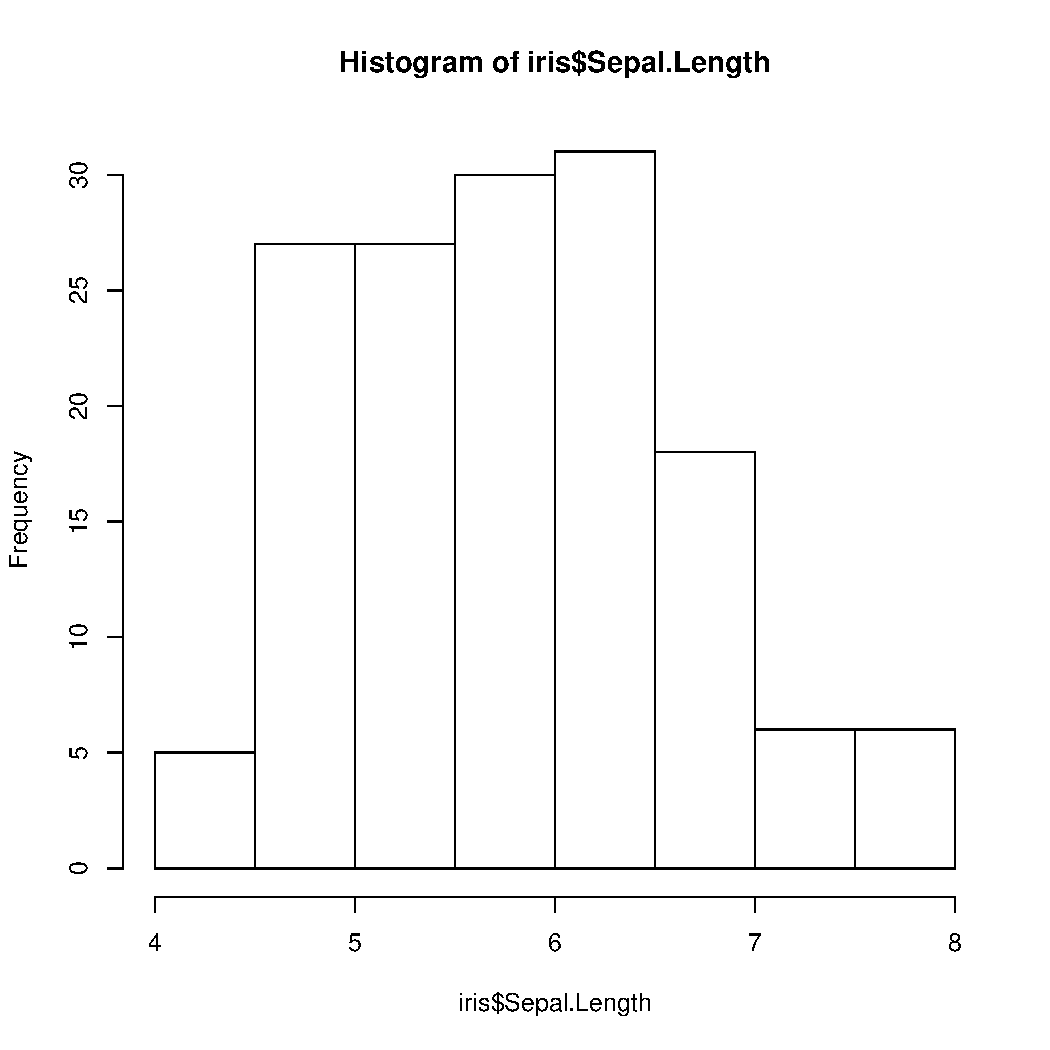
\includegraphics[width=\maxwidth]{figure/hist-1} 

\end{knitrout}

\begin{DIY}{Think}
Is the argument passed to $hist()$ a \emph{discrete attribute} or a \emph{continuous attribute}? Explain your choice.
\end{DIY}

\begin{DIY}{Think}
Change the histogram plot to show normalized frequencies
\end{DIY}

\subsubsection{The [] operator for sub-setting}
\begin{knitrout}
\definecolor{shadecolor}{rgb}{0.969, 0.969, 0.969}\color{fgcolor}\begin{kframe}
\begin{alltt}
\hlstd{iris}\hlopt{$}\hlstd{Sepal.Length[}\hlnum{1}\hlopt{:}\hlnum{10}\hlstd{]}
\end{alltt}
\begin{verbatim}
##  [1] 5.1 4.9 4.7 4.6 5.0 5.4 4.6 5.0 4.4 4.9
\end{verbatim}
\end{kframe}
\end{knitrout}

\begin{DIY}{Homework}
Find the sum of the first 10 and last 10 elements of the numeric array.
\end{DIY}

\subsubsection{The $plot()$ function}
\begin{knitrout}
\definecolor{shadecolor}{rgb}{0.969, 0.969, 0.969}\color{fgcolor}\begin{kframe}
\begin{alltt}
\hlkwd{plot}\hlstd{(cars}\hlopt{$}\hlstd{speed,cars}\hlopt{$}\hlstd{dist)}
\end{alltt}
\end{kframe}
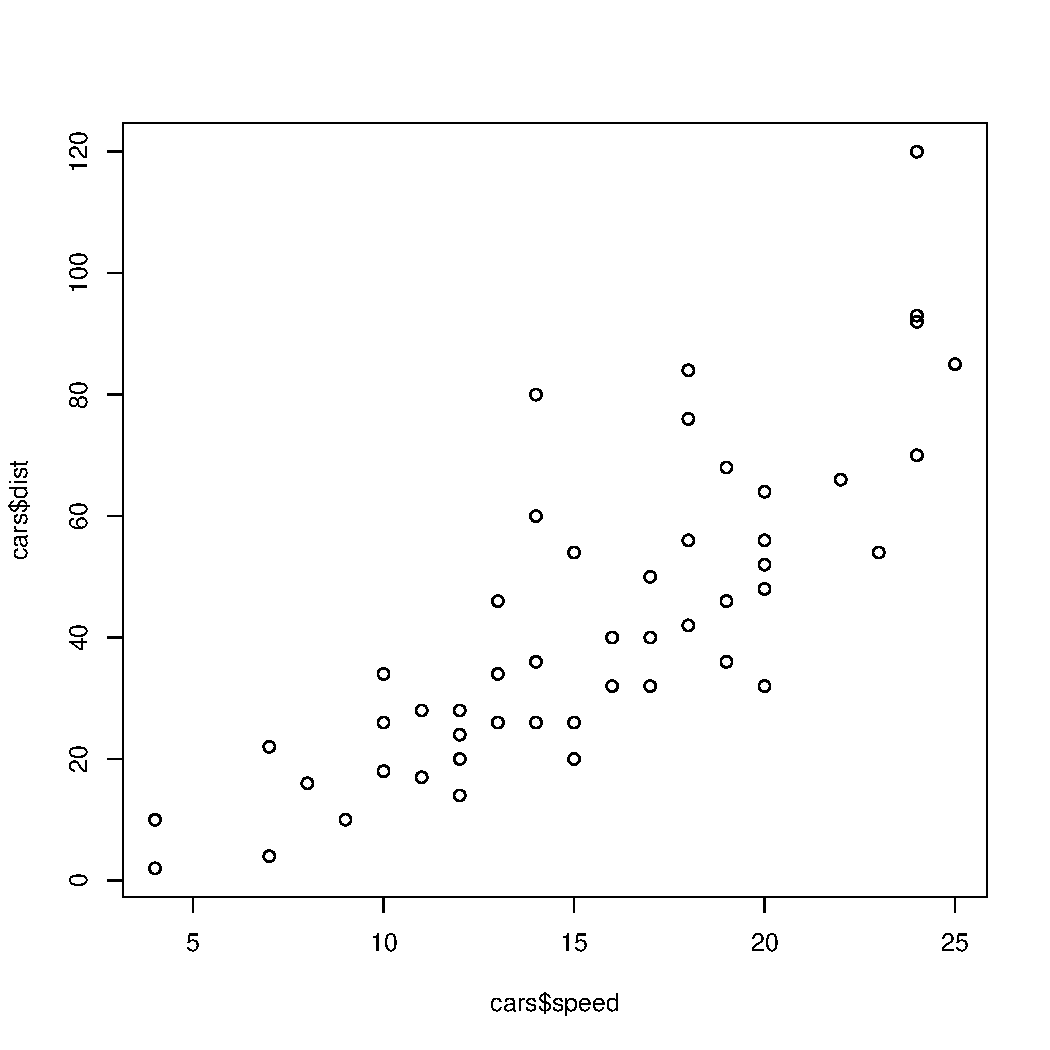
\includegraphics[width=\maxwidth]{figure/plot-1} 

\end{knitrout}

\begin{DIY}{Think}
Can you \emph{explain} the plot that you see above?
\end{DIY}

\begin{DIY}{Think}
Change the markers in the plot from circles to crosses. Moreover change the of the markers
\end{DIY}

\begin{DIY}{Homework}
Pick a dataset from the list of available datasets and \emph{explore it} using the \emph{R expressions} you have just learnt.
\end{DIY}

\subsection{Input/Output(I/O) with External Sources}
\subsubsection{IO with .txt files}
\subsubsection{IO with .csv files}
\subsubsection{IO with .xls files}
\subsubsection{IO with Relational Database Management Systems(RDBMS)}
